\section{Planarität}
\authors{Janek Paeßens und Charlotte Häußler}
\subsection{Definitionen und Motivation}
Im Folgenden soll die Planarität von Graphen behandelt werden, die relevante Anwendungen, wie auch eine interessante Theorie mit sich bringt. Planare Graphen sind Graphen, die sich überschneidungsfrei auf ein Blatt Papier zeichnen lassen. Beispiele für die Anwendung von planaren Graphen lassen sich im Chip-Design bzw. in der Platinen-Entwicklung finden, in der die Schaltkreise nur an möglichst wenigen Stellen Überschneidungen haben sollten.
\begin{df} Ein Graph $G=(V,E)$ heißt \textbf{planar}, wenn er sich so in die Ebene einbetten lässt, dass sich keine Kanten schneiden. \end{df}
Ob ein Graph planar ist oder nicht hängt dabei nicht von seiner Einbettung ab. Es ist also durchaus möglich, dass ein Graph trotz vorhandener Planarität mit Kantenüberschneidungen dargestellt wird.
\begin{df}Ein Graph heißt \textbf{maximal planar}, wenn er planar ist und keine weitere Kante hinzugefügt werden kann, ohne dass die Planarität zerstört wird.\end{df}
\begin{df}Ein \textbf{triangulierter Graph} ist ein planarer Graph der in einer spezifischen Einbettung nur aus Dreiecken besteht und auch in seiner Außenform ein Dreieck darstellt. \end{df}
In einem triangulierten Graphen bilden also alle Knoten mit ihren Nachbarknoten und den entsprechenden Kanten immer Dreiecke.


\subsection{Eigenschaften planarer Graphen}
Das folgende Lemma ist eine Aussage über planare Graphen, die dazu dient numerische Invarianten eines Graphens, in diesem Fall die Größe der Kanten- und Knotenmenge, miteinander in Beziehung zu setzen.
\begin{lemma}\label{lemma1}
Sei $G=(V,E)$ ein planarer Graph, der mindestens drei Knoten hat. Dann gilt
\begin{center}
$|E|\leq 3 \cdot |V| -6$.
\end{center}
\end{lemma}
\begin{proof}
Der Beweis geschieht mit Induktion über die Knotenanzahl $|V|$.  O.\,B.\,d.\,A. wird er nur für triangulierte Graphen durchgeführt werden. Triangulierte Graphen sind maximal planar und damit ist die Kantenanzahl im Verhältnis zur Knotenanzahl ebenfalls maximal. Somit wird nur der worst case betrachtet.\\ \\
Als Induktionsbeginn wird das obige Lemma für die kleinste betrachtete Knotenzahl $|V|=k=3$ gezeigt. Da $K_3$ der Graph ist, der für einen Graph mit $|V|=3$ die meisten Kanten, nämlich $|E|=3$ Kanten, besitzt wird dieser betrachtet. Setzt man die Werte dieses Falles in die Ungleichung $|E| \leq 3 \cdot |V| -6$ ein, so geht diese auf, da
\begin{align*}
3 \leq 3\cdot 3 -6.
\end{align*}
Die Induktionsvoraussetzung ist, dass für jeden triangulierten und planaren Graphen $G=(V,E)$ mit $|V|=k$ gilt
\begin{center}
$|E| \leq 3 \cdot |V| -6$.
\end{center}
Aus dieser Voraussetzung muss nun im Induktionsschritt gefolgert werden, dass die Aussage auch für einen beliebigen planaren Graphen mit $k+1$ Knoten gilt. Allerdings lassen sich nicht alle planaren triangulierten Graphen mit $k+1$ Knoten aus einem triangulierten Graphen mit $k$ Knoten konstruieren, indem ein Knoten und beliebig viele Kanten, die ihn mit den Knoten des Graphen verbinden, hinzugefügt werden. Deshalb wird von einem beliebigen Graphen $G=(V,E)$ mit $|V|=k+1$ Knoten ausgegangen und ein beliebiger Knoten $v\in V$ entfernt, sodass ein neuer Graph $G'=(V',E')$ mit $V'=V \: \backslash \:  \{v\}$ und $E'=E \: \backslash \: \{e\in E\: |\: v\in e\}$ entsteht. Damit die Induktionsvoraussetzung angewendet werden kann, muss $G'$ trianguliert werden. Hierzu wird eine Fallunterscheidung vorgenommen. \\
\begin{enumerate}
\item \textbf{$d(v)=3$: } In diesem Fall ist der Graph $G'$ bereits trianguliert, da von dem Knoten $v$ in $G$ nur drei Kanten ausgehen und so nach Entfernen des Knotens $v$ die drei ehemaligen Nachbarknoten von $v$ in $G'$ ein Dreieck bilden. Der Graph $G'$ ist daher weiterhin trianguliert, da er immer noch nur aus Dreiecken besteht.
\item \textbf{$d(v)>3$: } In diesem Fall muss man Kanten ergänzen, um den Graphen zu triangulieren. Durch das Löschen des Knotens $v$ bilden die zu $v$ in $G$ adjazenten\footnote{benachbart} Knoten $\{v_1, v_2, \cdots, v_{d(v)}\}$ in $G'$ ein $d(v)$-Eck. Dieses wird im Folgenden so ergänzt, dass sich ein triangulierter Graph $G''=(V'',E'')$ ergibt. Dabei muss man beachten, dass man keine bereits außerhalb des $d(v)$-Ecks durch eine Kante $e_{außen}$ verbundenen Knoten verbindet. Falls es keine solche Kante zwischen zwei Knoten des $d(v)$-Ecks gibt, so kann von einem beliebigen Punkt $v_j$ aus zu allen anderen Knoten des $d(v)$-Ecks bis auf $v_j$ und die zu $v_j$ adjazenten Knoten eine Kante ergänzt werden. Falls es doch mindestens eine solche Kante $e_{außen}$ gibt, wird eine Kante $e_{außen}=\{v_k,v_l\}$ betrachtet, für die die beiden Endpunkte $v_k, v_l\in V'$ die Knoten sind, die im $d(v)$-Eck die kürzeste Distanz zueinander haben. Durch diese spezifische Wahl wird garantiert, dass sich im Pfad innerhalb des $d(v)$-Ecks zwischen $v_k$ und $v_l$ keine Knoten befinden, die außerhalb des $d(v)$-Ecks durch eine Kante verbunden sind, da $e_{außen}$ bereits per Definition die kürzeste solcher Kanten ist. Ebenso können die Knoten, die im $d(v)$-Eck zwischen $v_k$ und $v_l$ liegen, zu keinem anderen Knoten außerhalb des Pfades durch eine außerhalb des $d(v)$-Ecks liegende Kante verbunden sein, da ein solcher Weg durch $e_{außen}$ blockiert wird. Daher kann ein beliebiger Knoten $v_{k\rightarrow l}$ von den Knoten, die im $d(v)$-Eck zwischen $v_k$ und $v_l$ liegen, mit allen anderen Knoten des $d(v)$-Ecks, bis auf die beiden Nachbarn und sich selbst, verbunden werden, um den Graphen zu triangulieren.  
\end{enumerate}
Für den Graphen $G''=(V'',E'')$ mit $|V''|=k$ gilt nach Induktionsvoraussetzung $|E''|\leq 3\cdot |V''|-6 $.
Beim Triangulieren werden genau $d(v)-3$ Kanten ergänzt, da alle Knoten bis auf $v_{k\rightarrow l}$  und seine Nachbarknoten mit $v_{k\rightarrow l}$ verbunden werden. Daher gilt die Beziehung $|E'|+d(v)-3=|E''|$. Weiterhin werden hierbei keine Knoten ergänzt oder entfernt, sodass $|V''|=|V'|$ gilt. Somit ergibt sich
\begin{equation}
\label{ungl}
|E'|+d(v)-3 \leq |V'|-6.
\end{equation}
Des Weiteren gilt, dass $|V|=|V'|+1$, da genau ein Knoten $v$ entfernt wurde. Da beim Entfernen dieses einen Knotens auch alle Kanten, die zu $v$ inzident sind, entfernt werden, gilt auch der Zusammenhang $|E|=|E'|+d(v)$. Setzt man dies in Ungleichung \ref{ungl} ein, so ergibt sich, was zu beweisen war.
\begin{align*}
&&|E|-d(v)+d(v)-3 &\leq 3\cdot (|V|-1)-6 \\
\Leftrightarrow &&|E|-3 &\leq 3\cdot |V|-9 \\
\Leftrightarrow &&|E|&\leq 3\cdot |V| -6 \qedhere
\end{align*}
\end{proof}
Aus dem nun bewiesenen Lemma ergibt sich eine weitere Eigenschaft planarer Graphen, die im Folgenden kurz erläutert und bewiesen werden soll.
\begin{korollar}\label{minimalgrad}
Sei $G=(V,E)$ ein planarer Graph. Dann gilt für seinen Minimalgrad $\delta (G)\leq 5$.
\end{korollar}
\begin{proof}
Da von jedem Knoten mindestens $\delta (G)$ Kanten ausgehen und die Summe aller Knotengrade eines Graphen das Doppelte der Kantenanzahl ist, gilt die Beziehung
\begin{center}
$\frac{1}{2} \cdot |V| \cdot \delta (G) \leq |E|$.
\end{center}
Zusammen mit Lemma \ref{lemma1} lässt sich schlussfolgern, dass
\begin{align*}
&&\frac{1}{2} \cdot |V| \cdot \delta (G) &\leq |E|\leq 3\cdot |V|-6 \\
\Leftrightarrow &&\delta (G) &\leq 6-\frac{12}{|V|} \\
\Rightarrow &&\delta(G)&\leq 5 \qedhere
\end{align*}
\end{proof}


\subsection{Spezielle nicht planare Graphen}
\begin{fakt} $K_5$ und $K_{3,3}$  (s. Abb. \ref{k33uk5}) sind nicht planar.\end{fakt} 
\begin{proof} Dass $K_5$ nicht planar ist, folgt direkt aus dem oben bewiesenen Lemma, da die Ungleichung $|E| \leq 3 \cdot |V| -6$ für die Werte von $K_5$ nicht gilt. \\
\begin{center}
$10 \not\leq 3\cdot 5 -6$
\end{center}
In $K_{3,3}$ wird ein Kreis der Länge sechs gesucht und o.\,B.\,d.\,A. dann planar in die Ebene eingebettet. Damit verbleiben noch genau drei Kanten, die es planar einzubetten gilt. Da diese drei Kanten aber die drei langen Diagonalen des Kreises sind, kann nur jeweils eine innerhalb und außerhalb des Kreises planar eingebettet werden. Somit ist in jedem Fall die planare Einbettung mindestens einer Kante und damit des gesamten Graphen nicht möglich. 
\end{proof}
\begin{figure}
	\centering
	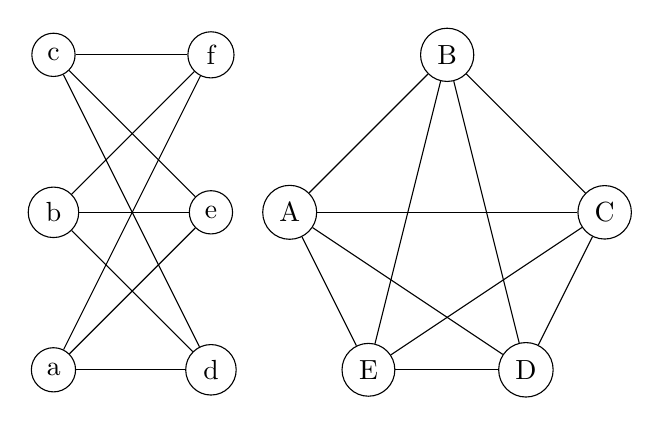
\begin{tikzpicture}
	\node[draw, circle](a) at (0,0){a};
	\node[draw, circle](b) at (0,2){b};
	\node[draw, circle](c) at (0,4){c};
	\node[draw, circle](d) at (2,0){d};
	\node[draw, circle](e) at (2,2){e};
	\node[draw, circle](f) at (2,4){f};
	\draw(a) -- (d);
	\draw(a) -- (e);
	\draw(a) -- (f);
	\draw(b) -- (f);
	\draw(b) -- (e);
	\draw(b) -- (d);
	\draw(c) -- (f);
	\draw(c) -- (e);
	\draw(c) -- (d);

	\node[draw, circle](A) at (3,2){A};
	\node[draw, circle](B) at (5,4){B};
	\node[draw, circle](C) at (7,2){C};
	\node[draw, circle](D) at (6,0){D};
	\node[draw, circle](E) at (4,0){E};
	\draw(A) -- (B);
	\draw(A) -- (C);
	\draw(A) -- (D);
	\draw(A) -- (E);
	\draw(B) -- (C);
	\draw(B) -- (D);
	\draw(B) -- (E);
	\draw(C) -- (D);
	\draw(C) -- (E);
	\draw(D) -- (E);

	\end{tikzpicture}
	\caption{Die Graphen $K_{3,3}$(links) und $K_5$(rechts)}
	\label{k33uk5}
\end{figure}
